\documentclass[10pt,leqno]{beamer}
\usecolortheme{UCA}
\usetheme{Warsaw}
\usepackage[default, scale=1.0]{lato}
\usepackage{amssymb,amsmath}

\usepackage[T1]{fontenc}
\usepackage[utf8]{inputenc}
\usepackage[spanish]{babel}

\usepackage{PDE} % mis definiciones
\renewcommand{\uu}{u}
\newcommand{\Nt}{N}
\newcommand{\Np}{{N_p}}
\newcommand{\interior}[1]{\mathring{#1}}
\newcommand{\refelem}{\widehat}

\usepackage{graphicx}
\hypersetup{breaklinks=true,
            bookmarks=true,
            pdfauthor={},
            pdftitle={},
            colorlinks=true,
            citecolor=blue,
            urlcolor=blue,
            linkcolor=magenta,
            pdfborder={0 0 0}}
\urlstyle{same}  % don't use monospace font for urls

%\usepackage{pifont} % checked mark
%\newcommand{\cmark}{\ding{51}}%
%\newcommand{\xmark}{\ding{55}}%


% ..........................................
% Bemer configuragion
% .........................................
% Quitar pie de página ....................
%gets rid of bottom navigation bars
\setbeamertemplate{footline}[frame number]{}


%gets rid of bottom navigation symbols
\setbeamertemplate{navigation symbols}{}

%empty header
\setbeamertemplate{headline}{}

%gets rid of footer
%will override 'frame number' instruction above
%comment out to revert to previous/default definitions
\setbeamertemplate{footline}{}

\AtBeginSection[]{
  %.............
  \begin{frame}
  \vfill
  \centering
  \begin{beamercolorbox}[sep=8pt,center,shadow=true,rounded=true]{title}
    \usebeamerfont{title}\insertsectionhead\par%
  \end{beamercolorbox}
  \vfill
  \end{frame}
}
\AtBeginSubsection{\frame{\subsectionpage}}

% Color for hyperlinks.....
\definecolor{links}{HTML}{0A5B31}
\hypersetup{colorlinks,linkcolor=,urlcolor=links}
%...........................................

\usepackage{amsthm}
\newtheorem{proposition}{Proposition}


\title{El Método de los Elementos Finitos}
\author{Rafa Rodríguez Galván}
\date{\today}

\begin{document}
\maketitle

\begin{frame}{Plan}

\begin{enumerate}
%\def\labelenumi{\arabic{enumi}.}
\setlength\itemsep{1em}
\item Formulación débil de EDP
\item Buen planteamiento del problema
\item Aproximación mediante el método de Galerkin
\item Estimaciones de error para el método de Galerkin
\item El método de los elementos finitos
\item Implementación en el ordenador
\end{enumerate}
\end{frame}


\begin{frame}{Conocimientos previos}
  Lo ideal sería tener una idea muy general sobre...
  \begin{itemize}
  \item Qué es un espacio de Hilbert
  \item Qué es la formulación variacional de una EDP
  \end{itemize}
% Dada una función \(f:\mathbb{R}\to \mathbb{R}\),
% \begin{block}{}
% \vspace{-1ex}
%   \[\mbox{hallar } \alpha\in\mathbb{R} \mbox{ tal que } f(\alpha)=0\]
% \end{block}
\end{frame}

\section{Formulación variacional de EDP}

\begin{frame}{Formulación variacional}
  \small
  Problema modelo: dado $\Omega\subset\mathbb{R}^n$, hallar
  $u\in V:=C^2(\Omega)$ tal que
  \begin{block}{}
    \vspace{-1.1ex}
    \begin{equation*}
      \left\{
        \label{eq:1}
        \begin{aligned}
          u - \Delta u &= f \quad\text{en } \Omega,  \\
          u | _{\partial\Omega} =& 0.
        \end{aligned}
      \right.
    \end{equation*}
  \end{block}

  \vfill
  Multiplicando por $v\in C^2(\Omega)$ e integrando por partes:
  \vspace{-1.0ex}
  \begin{block}{}
    \vspace{-1.1ex}
    \begin{equation*}
      \label{eq:2}
      \int_\Omega u\,v + \int_\Omega\grad u \grad v = \int_\Omega f\,v
      \quad\forall v\in V.
    \end{equation*}
  \end{block}

  \vfill
  \textbf{Problema variacional}: hallar
  $u\in V:= \{u\in C^1(\Omega),\ u|_{\partial\Omega}=0\}$ tal que
    \vspace{-1.0ex}
  \begin{block}{}
    \vspace{-2.9ex}
    \begin{equation}
      \label{eq:pb.variacional}
      \tag{P}
    a(u,v)= F(v) \quad \forall v \in V,
  \end{equation}
  \end{block}
  \vspace{1ex} donde
  $\displaystyle a(u,v)=\int_\Omega u\,v + \int_\Omega\grad u \grad v$
  \quad y \quad $\displaystyle F(v) = \int_\Omega f\,v$.
  \begin{itemize}
  \item Problema \textbf{mal planteado} en $V\sim C^2(\Omega)$ o
    $V \sim C^1(\Omega)$.
  \item \textbf{Idea}: tomar un espacio más amplio (que contiene a $C^1(\Omega)$):
  \begin{block}{}
    \vspace{-1ex}
    $$
    V:=H_0^1(\Omega).
    $$
  \end{block}
\end{itemize}
\end{frame}

\section{Buen planteamiento de problemas de contorno}
\label{sec:buen-plant-de}

\begin{frame}{Buen planteamiento de la formulación variacional}
  \textbf{Problema bien planteado} en el sentido de Hadamard:
  \begin{itemize}
  \item Existe una única solución
  \item Depende continuamente de los datos
  \end{itemize}

  \begin{block}{Teorema \textbf{Lax-Milgram}}
    Condición suficiente para que el
    problema~(\ref{eq:pb.variacional}) esté bien planteado:
    \begin{itemize}
    \item $V$ espacio de Hilbert
    \item $a(\cdot,\cdot)$ bilineal, continua, coerciva
    \item $F(\cdot)$ lineal continua (es decir, $F\in V'$)
    \end{itemize}
  \end{block}
\end{frame}

\section{Método de Galerkin}
\label{sec:buen-plant-de-1}

\begin{frame}{Problema aproximado}
  Dado $\Vh\subset V$ \textbf{finito-dimensional}, hallar $\uh\in\Vh$ tal que:
  \begin{block}{}
    \vspace{-2.5ex}
    \begin{equation}
      \label{eq:pb.aproximado}
      \tag{$P_h$}
      a(\uh,v)= F(v) \quad \forall \vh \in \Vh.
    \end{equation}
  \end{block}
  Resultados~(\cite{Brenner-Scott:08}, secciones 2.5, 2.8):
  \begin{itemize}
  \item Teorema: $\exists!$ solución de (\ref{eq:pb.aproximado})
  \item Proposición: el error es $a$--ortogonal a $\Vh$
  \item Lema de Céa: $\uh$ minimiza el error (en norma de energía, o
    sea norma en $V$):
    $$\norm[V]{u-\uh} \le \frac{C}{\alpha} min_{v\in\Vh}\norm[V]{u-v},$$
    siendo
    \begin{itemize}
    \item $C$ la constante de continuidad y
    \item $\alpha$ la constante de coercividad.
    \item Si $C$ ``grande'' o $\alpha$ ``pequeño'' $\Rightarrow$ problemas!!
    \end{itemize}
  \end{itemize}
\end{frame}

\begin{frame}{Método de Galerkin}
  Dado $\Vh\subset V$ \textbf{finito-dimensional}, hallar $\uh\in\Vh$ tal que:
  \begin{block}{}
    \vspace{-2.5ex}
    \begin{equation}
      \label{eq:pb.aproximado2}
      \tag{$P_h$}
      a(\uh,v)= F(v) \quad \forall \vh \in \Vh.
    \end{equation}
  \end{block}

  \textbf{Idea}:
  \begin{itemize}
  \item Fijar una base $\{\varphi_i\}_{i=1}^N$ de $\Vh$.
  \item Entonces,~(\ref{eq:pb.aproximado2}) se convierte en un sistema
    lineal de ecuaciones
    $$A\, U = b$$
  \item El vector $U$ contiene las coordenadas de la solución
    aproximada $\uh$ en la base $\{\varphi_i\}_{i=1}^N$:
    $$
    \uh(\xx) = \sum_{i=1}^N U_i \varphi_i(\xx)\quad\forall\xx\in\Omega.
    $$
  \item $\exists!$ solución del sistema anterior
  \end{itemize}
\end{frame}

\section{El método de los elementos Finitos}

\begin{frame}{El método de los elementos Finitos}
  \begin{center}
    % El método de los elementos Finitos
    % \\
    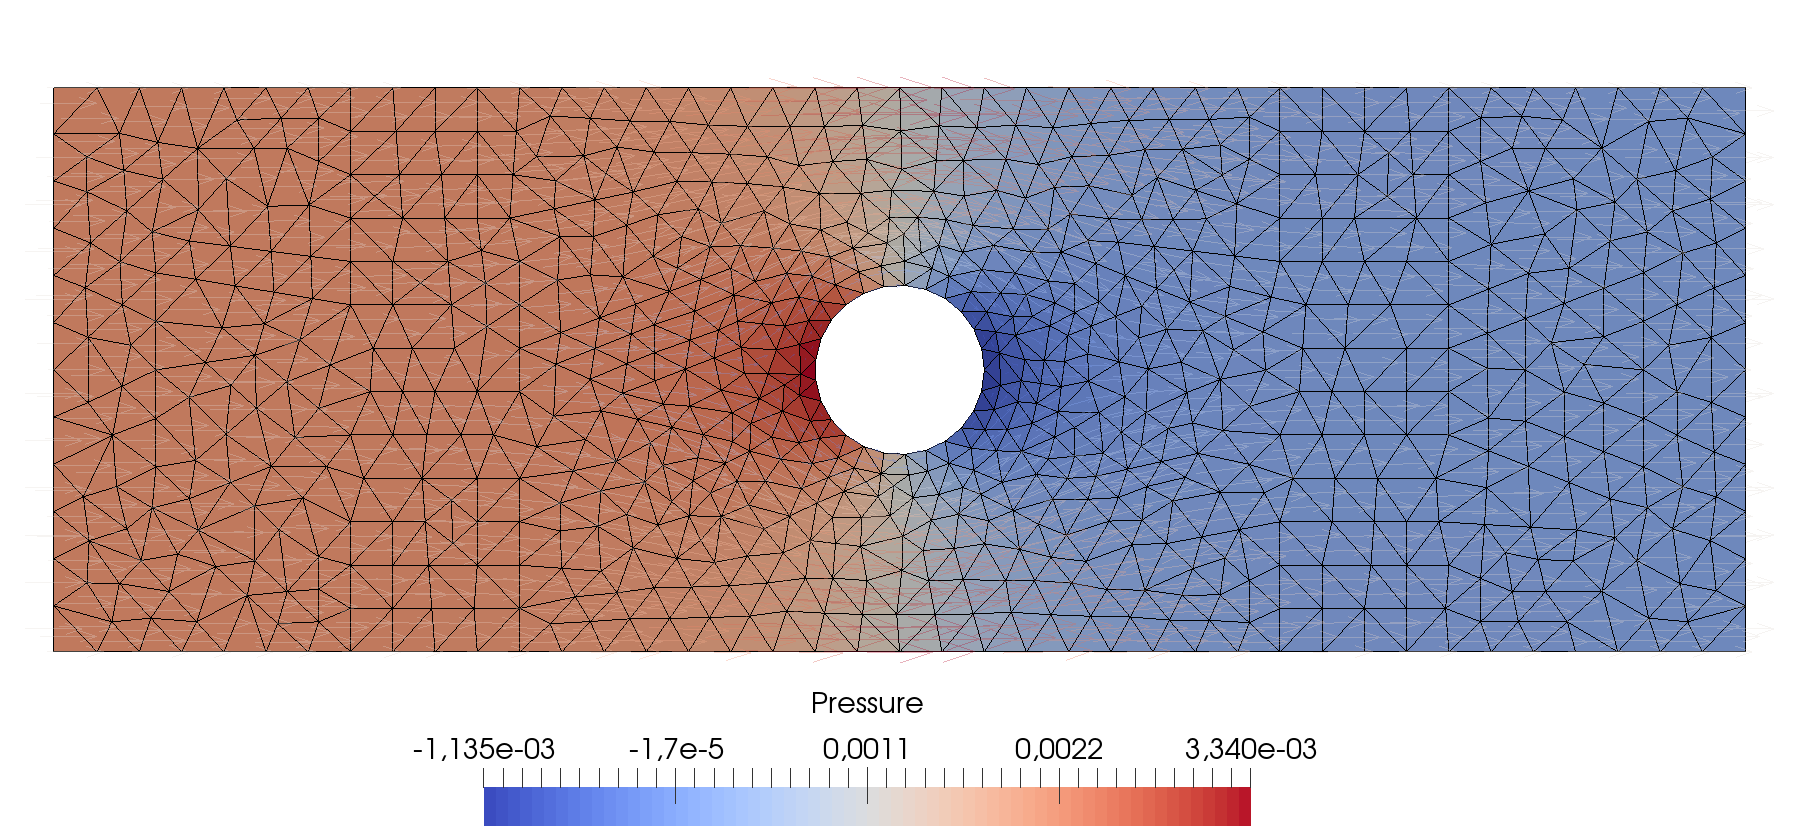
\includegraphics[width=0.99\linewidth]{mef}
  \end{center}
  \bigskip
  \textbf{Bibliografía}
  \small
  \begin{itemize}
  \item Ern-Guermond~\cite{Ern-Guermond:04}, capítulo 1
  \item Brenner-Scott~\cite{Brenner-Scott:08}, capítulo 3
  \item G. Allaire~\cite{allaire_numerical_2007}, capítulo 6
  \end{itemize}
\end{frame}


\begin{frame}{El método de los elementos Finitos}
  \vspace{-1.5em}
  \begin{flushright}
    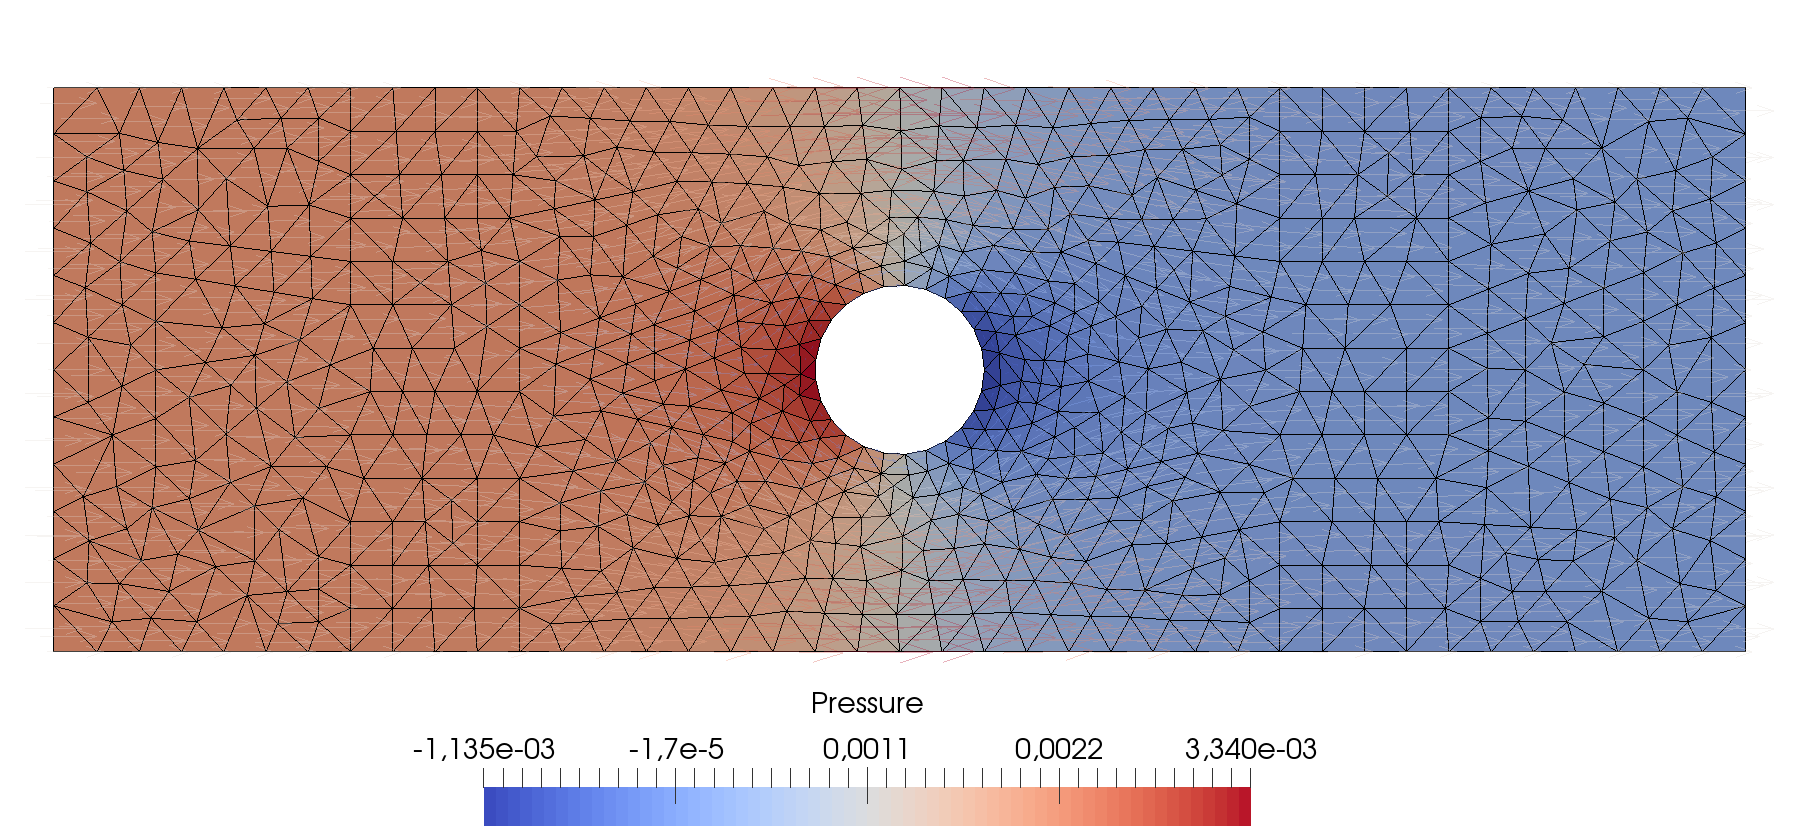
\includegraphics[width=0.4\linewidth]{mef}
  \end{flushright}
  \vspace{-3em}

  {\large \textbf{Idea}}:
  \bigskip
  \begin{enumerate}\itemsep1em
  \item Definir una <<\alert{\textit{triangulación}}>> (un mallado de $\Omega$)
    $$\Th=\{K_i\}_{i=1}^N \quad\text{ tal que }\quad
    \Omega\simeq\cup_{i=1}^n K_i
    $$
  \item En cada \textit{elemento}, $K$, aproximar la solución por un
    \alert{polinomio $\vh^K$}
  \item Definir un \alert{espacio global $\Vh$} finito-dimensional tal que
    \begin{flushright}
      \scriptsize (usualmente, $\Vh\subset C(\overline\Omega)$)
    \end{flushright}
    $$
    \forall \vh\in\Vh, \quad \vh|_K = \vh^K
    $$
  \item Aproximar la solución en $\Vh$ mediante el método de \alert{Galerkin}

  \item Lema de Céa $+$ Error en interpolación polinómica
    \begin{flushright}
      $\Rightarrow$ \alert{Estimaciones de error} para el MEF.
    \end{flushright}
  \end{enumerate}
\end{frame}

\subsection{Mallados o <<triangulaciones>>}

\begin{frame}{Mallado de $\Omega$}
  Supondremos:
  \bigskip
  \begin{itemize}\itemsep1em
  \item  $\Omega=\cup_{i=1}^\Nt K_i$, \quad
    $\interior{K_i}\cap\interior{K_j}=\emptyset$, $i\neq j$,
    \quad $K_i,K_j\in\Th$,
    \begin{flushright}
      \scriptsize
      donde $K_i$... \llaveizq{
        1d: intervalos
        \\[0.7ex]
        2d: polígonos (usualmente triángulos o rectángulos)
        \\[0.7ex]
        3d: poliedros (usualmente tetraedros o prismas)
        }
    \end{flushright}
  \item Todo $K\in\Th$ se puede obtener como transformación afín de un
    \alert{elemento de referencia} $\refelem K$:
    $$T_K: \refelem K \to K$$

  \item Hipótesis: <<\alert{elementos geométricamente conformes}>>\footnote{Ver e.g~\cite{Ern-Guermond:04}. Hipótesis fundamental para elementos finitos continuos}
    Dados dos elementos $K_i$, $K_j$ ($i\neq j$), entonces $K_i\cap K_j$ es:
    \begin{itemize}
    \item O bien vacío
    \item O bien un vértice, un lado o una cara común
    \end{itemize}
  \end{itemize}
\end{frame}


\subsection{Aproximación local por polinomios}

\begin{frame}{Definición abstracta de elemento finito}
  \begin{definition}[Ciarlet~\cite{Ciarlet:78}, Ern-Guermond~\cite{Ern-Guermond:04}]
    Un \textbf{\alert{Elemento finito}} en $\Rset^n$ es un triple
    $(K,P,\Sigma)$ tal que:
    \smallskip
    \begin{itemize}
    \item[(i)] \alert{$K$} = compacto de $\Rset^n$ con interior no vac\'io y
      frontera lipschtiziana
    \item[(ii)] \alert{$P$} = espacio de polinomios en $K$ de dimensi\'on $\Np+1$
    \item[(iii)] $\alert{\Sigma}=\{\sigma_0,\sigma_1,...,\sigma_{\Np}\} \subset V'$
      tales que la aplicaci\'on lineal
      \begin{align*}
        \sigma: P& \longrightarrow \mathbb{R}^{\Np+1},\\
        q& \longmapsto \sigma(q)=(\sigma_0(q), \sigma_1(q),..., \sigma_{\Np}(q))
      \end{align*}
      es biyectiva. Las formas lineales
      $\{\sigma_0,\sigma_1,...,\sigma_{\Np}\}$ se llaman
      \textit{grados de libertad} locales
    \end{itemize}
  \end{definition}

  \par\bigskip
  \scriptsize \textbf{Observación}:
  \par\medskip
  En ocasiones (por
  ejemplo~\cite{Ciarlet:78}) la biyectividad de $\sigma$ no se incluye
  en la definición de elemento finito. En ese caso, es una propiedad
  adicional y a los elementos que la verifican se les llama
  ``unisolventes''.
\end{frame}

\begin{frame}{Elementos finitos de Lagrange}

  \begin{definition} $(K,P,\Sigma)$ es un \alert{elemento finito de
      Lagrange} si sus grados de libertad están definidos de las siguiente
    forma:
    $$
    \sigma_i(p) := p(a_i), \quad \forall i=0,...,\Np,
    $$
    donde $\{a_0,...,a_\Np\} \subset K$ es un conjunto de puntos
    llamados <<\textbf{nodos}>>
  \end{definition}
\pause
\begin{proposition}
  \begin{enumerate}
  \item Existe una base $\{p_0,...,p_\Np\}$ de $P$ tal que
    $\sigma_i(p_j)=\delta_{ij}$
    \begin{flushright} \scriptsize $\hookrightarrow$  \alert{funciones base} locales
      (``\textit{local shape functions}'') del elemento finito
    \end{flushright}
  \item Todo $p\in P$ verifica: $p(x)=\sum_{i=0}^\Np \sigma_i(p) p_i(x)$
    \begin{flushright} \scriptsize $\hookrightarrow$ Es decir
      \alert{$(\sigma_0(p),\dots,\sigma_\Np(p))$ = coordenadas de
        $p(x)$ }en la base $\{p_0,...,p_\Np\}$
    \end{flushright}
  \end{enumerate}
\end{proposition}

\begin{footnotesize}
  \begin{enumerate}
  \item Demostración 1: Tomar $\{p_i\}$ = base de interpolación de
    Lagrange en el soporte $\{a_i\}$ % Entones
    % $\sigma_i(p_j)=p_j(a_i)=\delta_{ij}$
    \par
    Demostración 2: Consecuencia directa de la biyectividad de $\sigma$
    \item
    Unicidad de interpolación de valores $\sigma_i(p)$ en nodos $a_i$
  \end{enumerate}
\end{footnotesize}

\textbf{Observación}: \alert{esta proposición es válida para
  cualquier elemento finito} (no necesariamente de Lagrange)
\small
$\Leftarrow$ demostración~2
\end{frame}

\begin{frame}{Familia de elementos finitos de \textbf{Legendre}}
  \small
  \begin{itemize}
  \item Polinomios de Legendre (definición recursiva):
    \begin{footnotesize}
      \begin{align*}
        L_0(x)=1, \quad L_1(x)=x,
        \quad L_{k}(x) = \frac{2k-1}k L_{k-1}(x) - \frac{k-1}{k} L_{k-2}(x), \quad k\ge 2
      \end{align*}
    \end{footnotesize}
  \item $\{L_0,L_1,\dots,L_n\}$ base de
    $\mathbb{P}_n=\{\text{polinomios de grado } n\}$
  \item \alert{Base jerárquica}:
    $\{L_0,L_1,\dots,L_n\} \subset \{L_0,L_1,\dots,L_n, L_{n+1}\}$
  \item \alert{Ortogonalidad} en $\refelem K=[-1,1]$:
    \begin{footnotesize}
      $$\int_{-1}^1 L_i(x) L_j(x) = 2/(2i+1)\delta_{ij}$$
    \end{footnotesize}
  \item Extensión a intervalo $K$ arbitrario mediante la transformación afín
    $$T_K : \refelem K \to K$$
  \item Generalización a $K\subset\Rset^n$~\cite{solin_higher-order_2004}
  \end{itemize}
  \vspace{-0.3em}
  \normalsize
  \begin{definition} $(K,P,\Sigma)$ es un \alert{elemento finito de
      Legendre} si sus grados de libertad se definen como:
    $$
    \sigma_i(p) := \alpha_i, \quad \forall i=0,...,\Np,
    $$
    donde $(\alpha_0,...,\alpha_\Np) \in\Rset^{\Np+1}$ son las
    \vspace{-0.3em}
    \begin{center}
      \textbf{coordenadas} de $p(x)$ en la \textbf{base de Legendre}
      $\{L_0(x),...,L_\Np(x)\}$
    \end{center}
  \end{definition}

\end{frame}

\begin{frame}{Familia de elementos finitos de \textbf{Lobatto}}
  \small
  \begin{itemize}
  \item Polinomios de Lobatto (definición recursiva):
    \begin{footnotesize}
      \begin{align*}
        l_0(x)=\frac{1-x}2, \quad l_1(x)=\frac{1+x}2,
        \quad l_{k}(x) = \frac 1{\norm[L^2(\Omega)]{L_{k-1}}} \int_{-1}^x L_{k-1}(t) dt, \quad k\ge 2
      \end{align*}
    \end{footnotesize}
  \item $\{l_0,l_1,\dots,l_n\}$ base jerárquica de $\mathbb{P}_n$
  \item $\forall i\ge 0:$ \quad $l_i(-1)=0$ excepto \alert{$l_0(-1)=1$},
    \quad $l_i(1)=0$ excepto \alert{$l_1(1)=1$}
    \begin{flushright}
      \scriptsize
      $\hookrightarrow$ aplicación a \alert{continuidad} entre intervalos
    \end{flushright}
  \item $l'_k(x)=L_{k-1}(x) \Rightarrow$ \alert{ortogonalidad de $l'_i(x)$} en
    $\refelem K=[-1,1]$,
    \begin{footnotesize}
      $$\int_{-1}^1 l_i(x) l_j(x) = C\cdot \delta_{ij}, i,j\ge 2$$
    \end{footnotesize}

  \item \footnotesize Extensión a intervalo $K$ arbitrario mediante la transformación afín
    $$T_K : \refelem K \to K$$
  \item \footnotesize Generalización a $K\subset\Rset^n$~\cite{solin_higher-order_2004}
  \end{itemize}
  \vspace{-0.3em}
  \normalsize
  \begin{definition} $(K,P,\Sigma)$ es un \alert{elemento finito de
      Lobatto} si sus grados de libertad son:
    \vspace{-0.2em}
    $$
    \sigma_i(p) := \alpha_i, \quad \forall i=0,...,\Np,
    $$
    \vspace{-0.2em}
    donde $(\alpha_0,...,\alpha_\Np) \in\Rset^{\Np+1}$ son las
    \vspace{-0.2em}
    \begin{center}
      \textbf{coordenadas} de $p(x)$ en la \textbf{base de Lobatto}
      $\{L_0(x),...,L_\Np(x)\}$
    \end{center}
  \end{definition}
\end{frame}

\begin{frame}{Familia de elementos finitos de \textbf{Bernstein}}
  \small
  \begin{itemize}
  \item Polinomios de Bernstein
    \begin{footnotesize}
      $$
      b_k^n(x) = \binom{n}{k} (1-x)^{n-k} x^k, \quad k=0,...,n
      $$
    \end{footnotesize}
  \item $\{b_0^n,b_1^n,\dots,b_n^n\}$ base \emph{no jerárquica} pero
    \alert{positiva} de $\mathbb{P}_n$ en $\refelem K=[0,1]$
  \item $\forall i\ge 0:$ \quad $b_i^n(0)=0$ excepto \alert{$b_0^n(0)=1$},
    \quad $b_i^n(1)=0$ excepto \alert{$b_n^n(1)=1$}
    \begin{flushright}
      \scriptsize
      $\hookrightarrow$ aplicación a \alert{continuidad} entre intervalos
    \end{flushright}

  \item \footnotesize Extensión a intervalo $K$ arbitrario mediante la transformación afín
    $$T_K : \refelem K \to K$$
  \item \footnotesize Generalización a $K\subset\Rset^n$~\cite{solin_higher-order_2004}
  \end{itemize}
 \vspace{-0.3em}
  \normalsize
  \begin{definition} $(K,P,\Sigma)$ es un \alert{elemento finito de
      Bernstein} si sus grados de libertad son:
    \vspace{-0.2em}
    $$
    \sigma_i(p) := \alpha_i, \quad \forall i=0,...,\Np,
    $$
    \vspace{-0.2em}
    donde $(\alpha_0,...,\alpha_\Np) \in\Rset^{\Np+1}$ son las
    \vspace{-0.2em}
    \begin{center}
      \textbf{coordenadas} de $p(x)$ en la \textbf{base de Bernstein}
      $\{b_0^{\Np}(x),...,b_\Np^{\Np}(x)\}$
    \end{center}
  \end{definition}
\end{frame}

\subsection{Espacios globales de elementos finitos}

\begin{frame}{Elementos discontinuos}
  \begin{itemize}
  \item Construir espacios de elementos discontinuos es fácil:
  $$
  V_h^{dc} = \{ \vh\in \alert{L^2(\Omega)},\ /\ \vh|_K \in
  \mathbb{P}_n\ \forall K\in\Th\}
  $$
\item
  Para aplicar Galerkin necesito una base.
  \begin{itemize}
  \item Fijamos una base local $\{\varphi_i^K\}_{i=0}^{\Np}$ en cada
    $K\in \Th$
  \item Definimos la base global
    $\{\varphi_{i,k}\}_{i=1...\Np, j=1...\Nt}$ como
    \begin{equation*}
      \varphi_{i,k}(x) = \left\{
        \begin{aligned}
          \varphi_i^{K_k} (x) &\quad \text{si } x\in K_k \\
          0 &\quad \text{en otro caso}
        \end{aligned}
      \right.
    \end{equation*}
  \end{itemize}
\item Ventaja: simplicidad, más fácil el cálculo paralelo
\item Inconveniente método no conforme, es decir:
  $$\Vh\not\subset H^1(\Omega)$$
  luego
  $$
  \Vh \not\subset V\subset H^1(\Omega)
  $$
 luego \textbf{no} se puede aplicar \textbf{directamente} el \textbf{método de Galerkin}
\end{itemize}
\end{frame}

\begin{frame}{Elementos continuos}
  \begin{itemize}
  \item Construir espacios de elementos discontinuos es más difícil:
  $$
  V_h^{dc} = \{ \vh\in \alert{C(\Omega)},\ /\ \vh|_K \in
  \mathbb{P}_n\ \forall K\in\Th\}
  $$
\item
  Para aplicar Galerkin necesito una base.
  \begin{itemize}
  \item Fijamos una base local $\{\varphi_i^K\}_{i=0}^{\Np}$ en cada
    $K\in \Th$
  \item Definimos la base global
    $\{\varphi_{i,k}\}_{i=1...\Np, j=1...\Nt}$ como
    \begin{equation*}
      \varphi_{i,k}(x) = \left\{
        \begin{aligned}
          \varphi_i^{K_k} (x) &\quad \text{si } x\in K_k \\
          0 &\quad \text{en otro caso}
        \end{aligned}
      \right.
    \end{equation*}
  \item \alert{Exigimos que la base global sea \textbf{continua}}
  \end{itemize}
\item Inconveniente:  más difícil construir las funciones base, cálculo paralelo más complejo
\item Ventaja: método conforme, puede aplicar directamente el
  \textbf{método de Galerkin}
\end{itemize}
\end{frame}

\bibliography{biblio}{}
\bibliographystyle{alpha}   %{plain}

\end{document}
